\documentclass{standalone}
    \usepackage{tikz}
    \usetikzlibrary{matrix,chains,positioning,decorations.pathreplacing,arrows}
    \begin{document}
    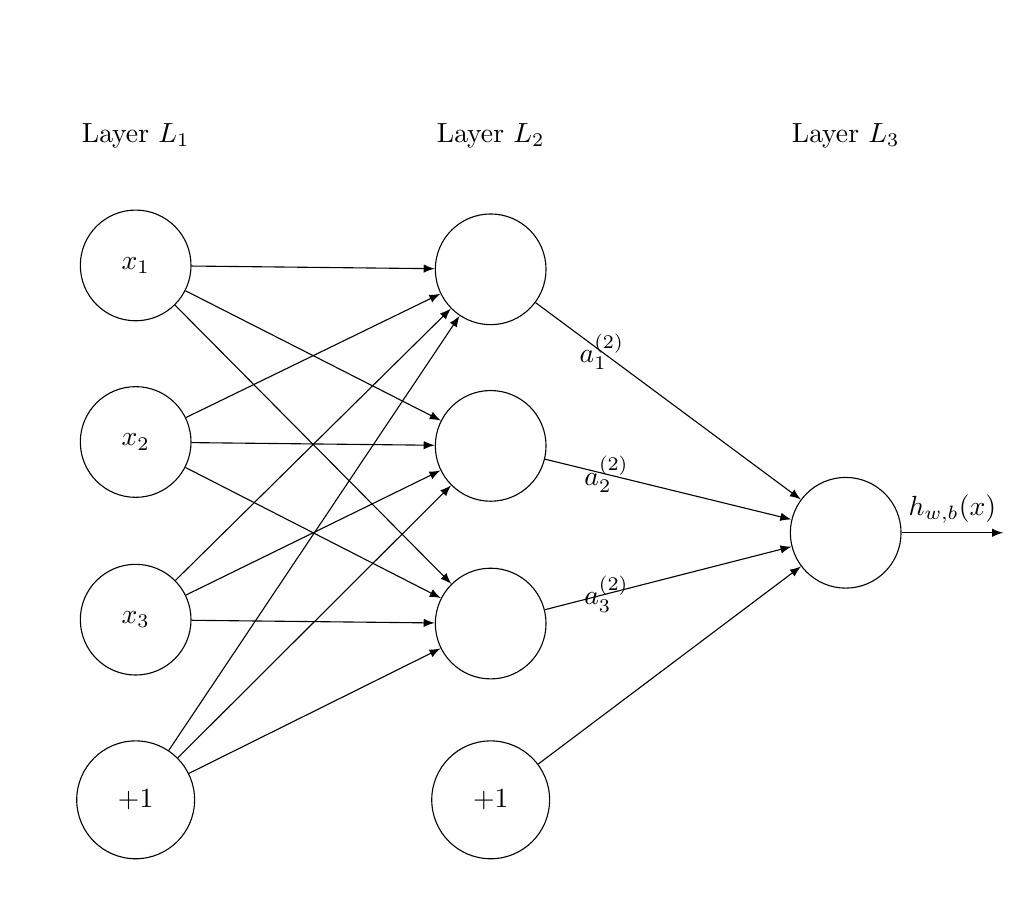
\begin{tikzpicture}[
        plain/.style={
          draw=none,
          fill=none,
          },
        net/.style={
          matrix of nodes,
          nodes={
            draw,
            circle,
            inner sep=10pt,
            minimum size=40pt
            },
          nodes in empty cells,
          column sep=2cm,
          row sep=-9pt
          },
        >=latex
        ]
        \matrix[net] (mat)
        {
        |[plain]| \parbox{1.6cm}{\centering Layer $L_1$} & |[plain]| \parbox{1.6cm}{\centering Layer $L_2$} & |[plain]| \parbox{1.6cm}{\centering Layer $L_3$} \\
        $x_1$& & |[plain]| \\
        |[plain]| & |[plain]| \\        
        $x_2$& & |[plain]| \\
        |[plain]| & |[plain]| &\\
        $x_3$& & |[plain]| \\
        |[plain]| & |[plain]| \\
        $+1$& $+1$ & |[plain]| \\   };
        % \foreach \ai [count=\mi ]in {2,4,6}
            % node at (mat-\ai-1) {$x_\mi$};
        %   \draw[<-] (mat-\ai-1) -- node {Input \mi} +(-2cm,0);
        \foreach \ai in {2,4,...,8}
        {\foreach \aii in {2,4,6}
          \draw[->] (mat-\ai-1) -- (mat-\aii-2);
        }
        \foreach \ai [count=\mi] in {2,4,...,6}
          \draw[->] (mat-\ai-2) -- node[near start] {$a_\mi^{(2)}$} (mat-5-3);
          \draw[->] (mat-8-2) -- (mat-5-3);
          \draw[->] (mat-5-3) -- node[above] {$h_{w,b}(x)$} +(2cm,0);
        \end{tikzpicture}
    \end{document}